\begin{mainquestion}{resistor_code}{Resistor Code}

An intrepid engineering student scoured through the lab64 miscellaneous parts bin and found two resistors shown here, both with values specified at 25 °C.  The first is a carbon film resistor rated to 1W with a TCR of −350ppm/°C; the second is a metal film resistor rated to ¼ W with a TCR of +50ppm/°C.  The student wishes to make use of these in a circuit which is to be placed in an unregulated temperature environment where the ambient temperature could potentially fluctuate anywhere between 5 °C and 40 °C.

\begin{figure}[htbp]
    \centering
    % Left Image (No Caption)
    \begin{minipage}[b]{0.3\textwidth}
        \centering
        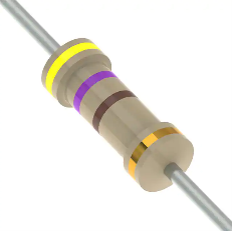
\includegraphics[width=\textwidth]{img_r1.png}
    \end{minipage}
    \begin{minipage}[b]{0.3\textwidth}
        \centering
        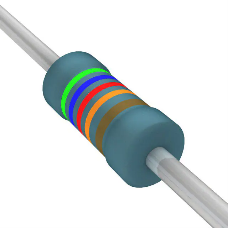
\includegraphics[width=\textwidth]{img_r2.png}
    \end{minipage}
\end{figure}

% =========================================================
\begin{partquestion}{minmax}
{For each resistor, what are the minimum and maximum expected values for the actual resistance?}

\begin{answer}
First, let us identify the nominal values (measured at \qty{25}{\celsius}) for each resistor using the color codes. The first is a four-band resistor with the first two bands (yellow: 4 and violet: 7) giving the value of 47, and the third band (brown: 1) as the multiplier giving the value of $10^1=10$. The first resistor is therefore a \qty{470}{\ohm} resistor. Note the tolerance is stated to be 5\% based on the gold band in the fourth position. The second is a five-band resistor, with the first three bands (green: 5, blue: 6 and red: 2) giving the value of 562, and the fourth band (orange: 3) as the multiplier giving the value of $10^3=1000$. The first resistor is therefore a \qty{562}{\kilo\ohm} resistor. Note the tolerance is stated to be 1\% based on the brown band in the fifth position. There are two factors which contribute possible deviation from nominal values. The first is the tolerance of the resistor, which means the actual room temperature value could deviate from the stated value. The second is the environmental temperature swings which can cause the resistance to go up or down.

Starting with the first resistor, the tolerance alone could produce a minimum resistance of

\[
R_{1,\mathrm{bot}}
=
\qty{470}{\ohm}\left(0.95\right)
=
\qty{446.5}{\ohm},
\]

and a maximum of

\[
R_{1,\mathrm{top}}
=
\qty{470}{\ohm}\left(1.05\right)
=
\qty{493.5}{\ohm}.
\]

On top of these values, we could see temperature deviations of at most \qty{-20}{\celsius} and \qty{15}{\celsius} from room temperature (\qty{25}{\celsius}). Because of the negative TCR found in carbon film resistors, a drop in temperature will result in an increase in resistance through the equation:

\[
R=R_0\left(1+\mathrm{TCR}\cdot\Delta T\right).
\]

At the bottom tolerance boundary, this becomes:

\[
R_{1,\mathrm{bot,highT}}
=
\left(\qty{446.5}{\ohm}\right)
\left(1-0.000350\left(15\right)\right)
=
\qty{444.2}{\ohm}
\]

\[
R_{1,\mathrm{bot,lowT}}
=
\left(\qty{446.5}{\ohm}\right)
\left(1-0.000350\left(-20\right)\right)
=
\qty{449.6}{\ohm}
\]

At the top tolerance boundary, this becomes:

\[
R_{1,\mathrm{top,highT}}
=
\left(\qty{493.5}{\ohm}\right)
\left(1-0.000350\left(15\right)\right)
=
\qty{490.9}{\ohm}
\]

\[
R_{1,\mathrm{top,lowT}}
=
\left(\qty{493.5}{\ohm}\right)
\left(1-0.000350\left(-20\right)\right)
=
\qty{497.0}{\ohm}
\]

Examining the four results reveals that

\[
R_{\mathrm{min}}
=
R_{1,\mathrm{bot,highT}}
=
\qty{444.2}{\ohm}
\]

and

\[
R_{\mathrm{max}}
=
R_{1,\mathrm{top,lowT}}
=
\qty{497.0}{\ohm}.
\]

Considering now the second resistor, the tolerance alone could produce a minimum resistance of

\[
R_{2,\mathrm{bot}}
=
\qty{562}{\kilo\ohm}\left(0.99\right)
=
\qty{556.4}{\kilo\ohm},
\]

and a maximum of

\[
R_{2,\mathrm{top}}
=
\qty{562}{\kilo\ohm}\left(1.01\right)
=
\qty{567.6}{\kilo\ohm}.
\]

On top of these values, we could see temperature deviations of at most \qty{-20}{\celsius} and \qty{15}{\celsius} from room temperature (\qty{25}{\celsius}). Because of the positive TCR found in metal film resistors, a drop in temperature will result in a decrease in resistance through the equation:

\[
R=R_0\left(1+\mathrm{TCR}\cdot\Delta T\right).
\]

At the bottom tolerance boundary, this becomes:

\[
R_{2,\mathrm{bot,highT}}
=
\left(\qty{556.4}{\kilo\ohm}\right)
\left(1+0.000050\left(15\right)\right)
=
\qty{556.8}{\kilo\ohm}
\]

\[
R_{2,\mathrm{bot,lowT}}
=
\left(\qty{556.4}{\kilo\ohm}\right)
\left(1+0.000050\left(-20\right)\right)
=
\qty{555.8}{\kilo\ohm}
\]

At the top tolerance boundary, this becomes:

\[
R_{2,\mathrm{top,highT}}
=
\left(\qty{567.6}{\kilo\ohm}\right)
\left(1+0.000050\left(15\right)\right)
=
\qty{568.0}{\kilo\ohm}
\]

\[
R_{2,\mathrm{top,lowT}}
=
\left(\qty{567.6}{\kilo\ohm}\right)
\left(1+0.000050\left(-20\right)\right)
=
\qty{567.1}{\kilo\ohm}
\]

Examining the four results reveals that

\[
R_{\mathrm{min}}
=
R_{2,\mathrm{bot,lowT}}
=
\qty{555.8}{\kilo\ohm}
\]

and

\[
R_{\mathrm{max}}
=
R_{2,\mathrm{top,highT}}
=
\qty{568.0}{\kilo\ohm}.
\]
\end{answer}
\end{partquestion}

% =========================================================
\begin{partquestion}{maxvolt}
{Based on your result from (\cref{prob:resistor_code:minmax}), for each resistor, what is the maximum voltage that could be applied to ensure the stated power rating is not exceeded? Ignore any effects of thermal resistance due to the heat dissipated in the resistors.}

\begin{answer}

Because
\[
P=\frac{V^2}{R},
\]
the maximum voltage possible under all conditions is the one that can be met with the smallest $R$. Therefore, for the carbon film resistor:

\[
\qty{1}{\watt}
=
\frac{V^2}{\qty{444.2}{\ohm}}.
\]

From which it follows that

\[
V
<
\sqrt{\left(\qty{444.2}{\ohm}\right)\left(\qty{1}{\watt}\right)}
=
\qty{21.08}{\volt}.
\]

For the metal film resistor:

\[
\qty{0.25}{\watt}
=
\frac{V^2}{\qty{555.8}{\kilo\ohm}}.
\]

From which it follows that

\[
V
<
\sqrt{\left(\qty{555.8}{\kilo\ohm}\right)\left(\qty{0.25}{\watt}\right)}
=
\qty{372.76}{\volt}.
\]

\end{answer}
\end{partquestion}

% =========================================================
\begin{partquestion}{thermal_resistance}
{Repeat part (\cref{prob:resistor_code:maxvolt}) assuming an overall thermal resistance of \qty{0.25}{\kelvin\per\milli\watt} for each resistor.}

\begin{answer}

We can ignore the top boundary of the resistor tolerance because the smaller values of resistance are found at the bottom boundary. If we denote the power being dissipated in the resistor as $P$ watts, and we drive a resistor with a nominal value $R_{0,\mathrm{bot}}$ at the bottom end of the tolerance boundary, we can write

\[
R
=
R_{0,\mathrm{bot}}
\left(
1+\mathrm{TCR}
\left(
\Delta T
+
P\cdot250
\right)
\right).
\]

The power dissipated in the resistor is

\[
P
=
\frac{V^2}{R}
=
\frac{V^2}
{R_{0,\mathrm{bot}}
\left(
1+\mathrm{TCR}
\left(
\Delta T
+
P\cdot250
\right)
\right)}.
\]

For the carbon-film resistor, the worst case will be when the temperature is highest. The maximum voltage can be solved for when $P=\qty{1}{\watt}$:

\def\power{\qty{1}{\watt}}
\begin{align*}
V &= \sqrt{P \cdot R_{0,\mathrm{bot}}\left(1+\mathrm{TCR}\left(\Delta T+P\cdot250\right)\right)} \\
V_{\text{max}} &= \sqrt{\power \cdot \qty{446.5}{\ohm}\left(1+\qty{0.000350}{\per\celsius}\left(\qty{15}{\celsius}+\power \cdot\qty{250}{\celsius\per\watt}\right)\right)} \\
V_{\text{max}} &= \qty{20.1}{\volt}
\end{align*}

For the metal-film resistor, the worst case will be when the temperature is lowest. The maximum voltage can be solved for when $P=\qty{0.25}{\watt}$:

\def\power{\qty{0.25}{\watt}}
\begin{align*}
V &= \sqrt{P \cdot R_{0,\mathrm{bot}}\left(1+\mathrm{TCR}\left(\Delta T+P\cdot250\right)\right)} \\
V_{\text{max}} &= \sqrt{\power \cdot \qty{556.4}{\kilo\ohm}\left(1+\qty{0.000050}{\per\celsius}\left(\qty{-20}{\celsius}+\power \cdot\qty{250}{\celsius\per\watt}\right)\right)} \\
V_{\text{max}} &= \qty{373.4}{\volt}
\end{align*}

\end{answer}
\end{partquestion}
\end{mainquestion}